\chapter{Discussion}

% Start with the big picture.
Our analysis of the Orion A and Orion B molecular clouds reveals a complex interplay between morphology, topology, and star formation activity. 
By combining perimeter–area scaling, Euler characteristic profiles, and mass–size relations, we obtain a consistent picture of how structural complexity varies across column densities and how these variations relate to the presence of young stellar objects.

% Synthesize the fractal dimension results (global and local).
% To-Do:
% Visuals
The global fractal dimension is based on the idea that, if a structure is self-similar i.e lacks a particular characteristic scale, perimeter and area of the structure at all scale should scale linearly in a log-log diagram. 
Turbulence in clouds is a known player for the organization of structures, and this set of tool is helping us identifying how much this self-similar behaviour influences the structures.

This global perimeter–area analysis reveals distinct structural regimes within Orion~A, with a clear transition in slope that reflects different complexity regimes at low and high column densities.  
In contrast, Orion~B maintains a more uniform fractal signature.  
This contrast already begins to paint a picture in which Orion~A and Orion~B are governed by different physical conditions.

For Orion~A, a double fit is required, indicating a change in the underlying physics.  
This transition occurs at a column density of \(N = 1.23 \times 10^{22}\,\mathrm{cm}^{-2}\), marking a physically significant scale.  
At this threshold, the structural properties of Orion~A shift, coinciding with the onset of active star formation and the emergence of dense cores \cite{lada2010star}.  
The change in fractal dimension and topology at this scale suggests a direct link between the cloud's morphology and the physical processes driving star formation.

In Orion~B, no such break is necessary.  
This outcome is broadly consistent with expectations, as Orion~B is known to be a more turbulent molecular cloud.  
In such an environment, scale‑free behavior dominates over the column‑density range analyzed, which is reflected in the high quality of the single global fractal dimension fit.  
Together, these findings establish the first elements of a coherent picture described by the Minkowski functionals.

The local fractal dimension takes instead the base of the perimeter-area relation and inverse it to obtain a proxy for the complexity of single structures.
This picture is a bit more complex, but more faceted as well.

% Integrate topological insights (Euler characteristic).
% To-Do:
% Remake Images (after making sure that the definition is correct)
Furthermore, the Euler characteristic highlights clear differences between Orion~A and Orion~B.  
Orion~A exhibits a profile that closely resembles the behavior expected from Gaussian Random Field simulations, with a well-defined peak at approximately \(1.64 \times 10^{22}\,\mathrm{cm}^{-2}\).  
This threshold is significant, echoing the transition seen in the global fractal dimension analysis, and marks the emergence of dense cores within the cloud.

In contrast, Orion~B shows no such pronounced peak, instead displaying a more gradual, almost linear decrease.  
If Orion~B is indeed more strongly influenced by turbulence, this behavior is consistent with a more scale-free, less clustered structure, where the appearance of dense cores is more gradual and widely distributed.  
The topological analysis therefore reinforces the notion that turbulence governs the structural evolution of Orion~B, while Orion~A undergoes distinct transitions closely tied to star-formation thresholds.

Visual examples of the changes in the Euler characteristic for Orion~A and Orion~B are provided in Figures~\ref{fig:Euler_Orion_A} and~\ref{fig:Euler_Orion_B}.

\begin{figure}[t]
    \centering
    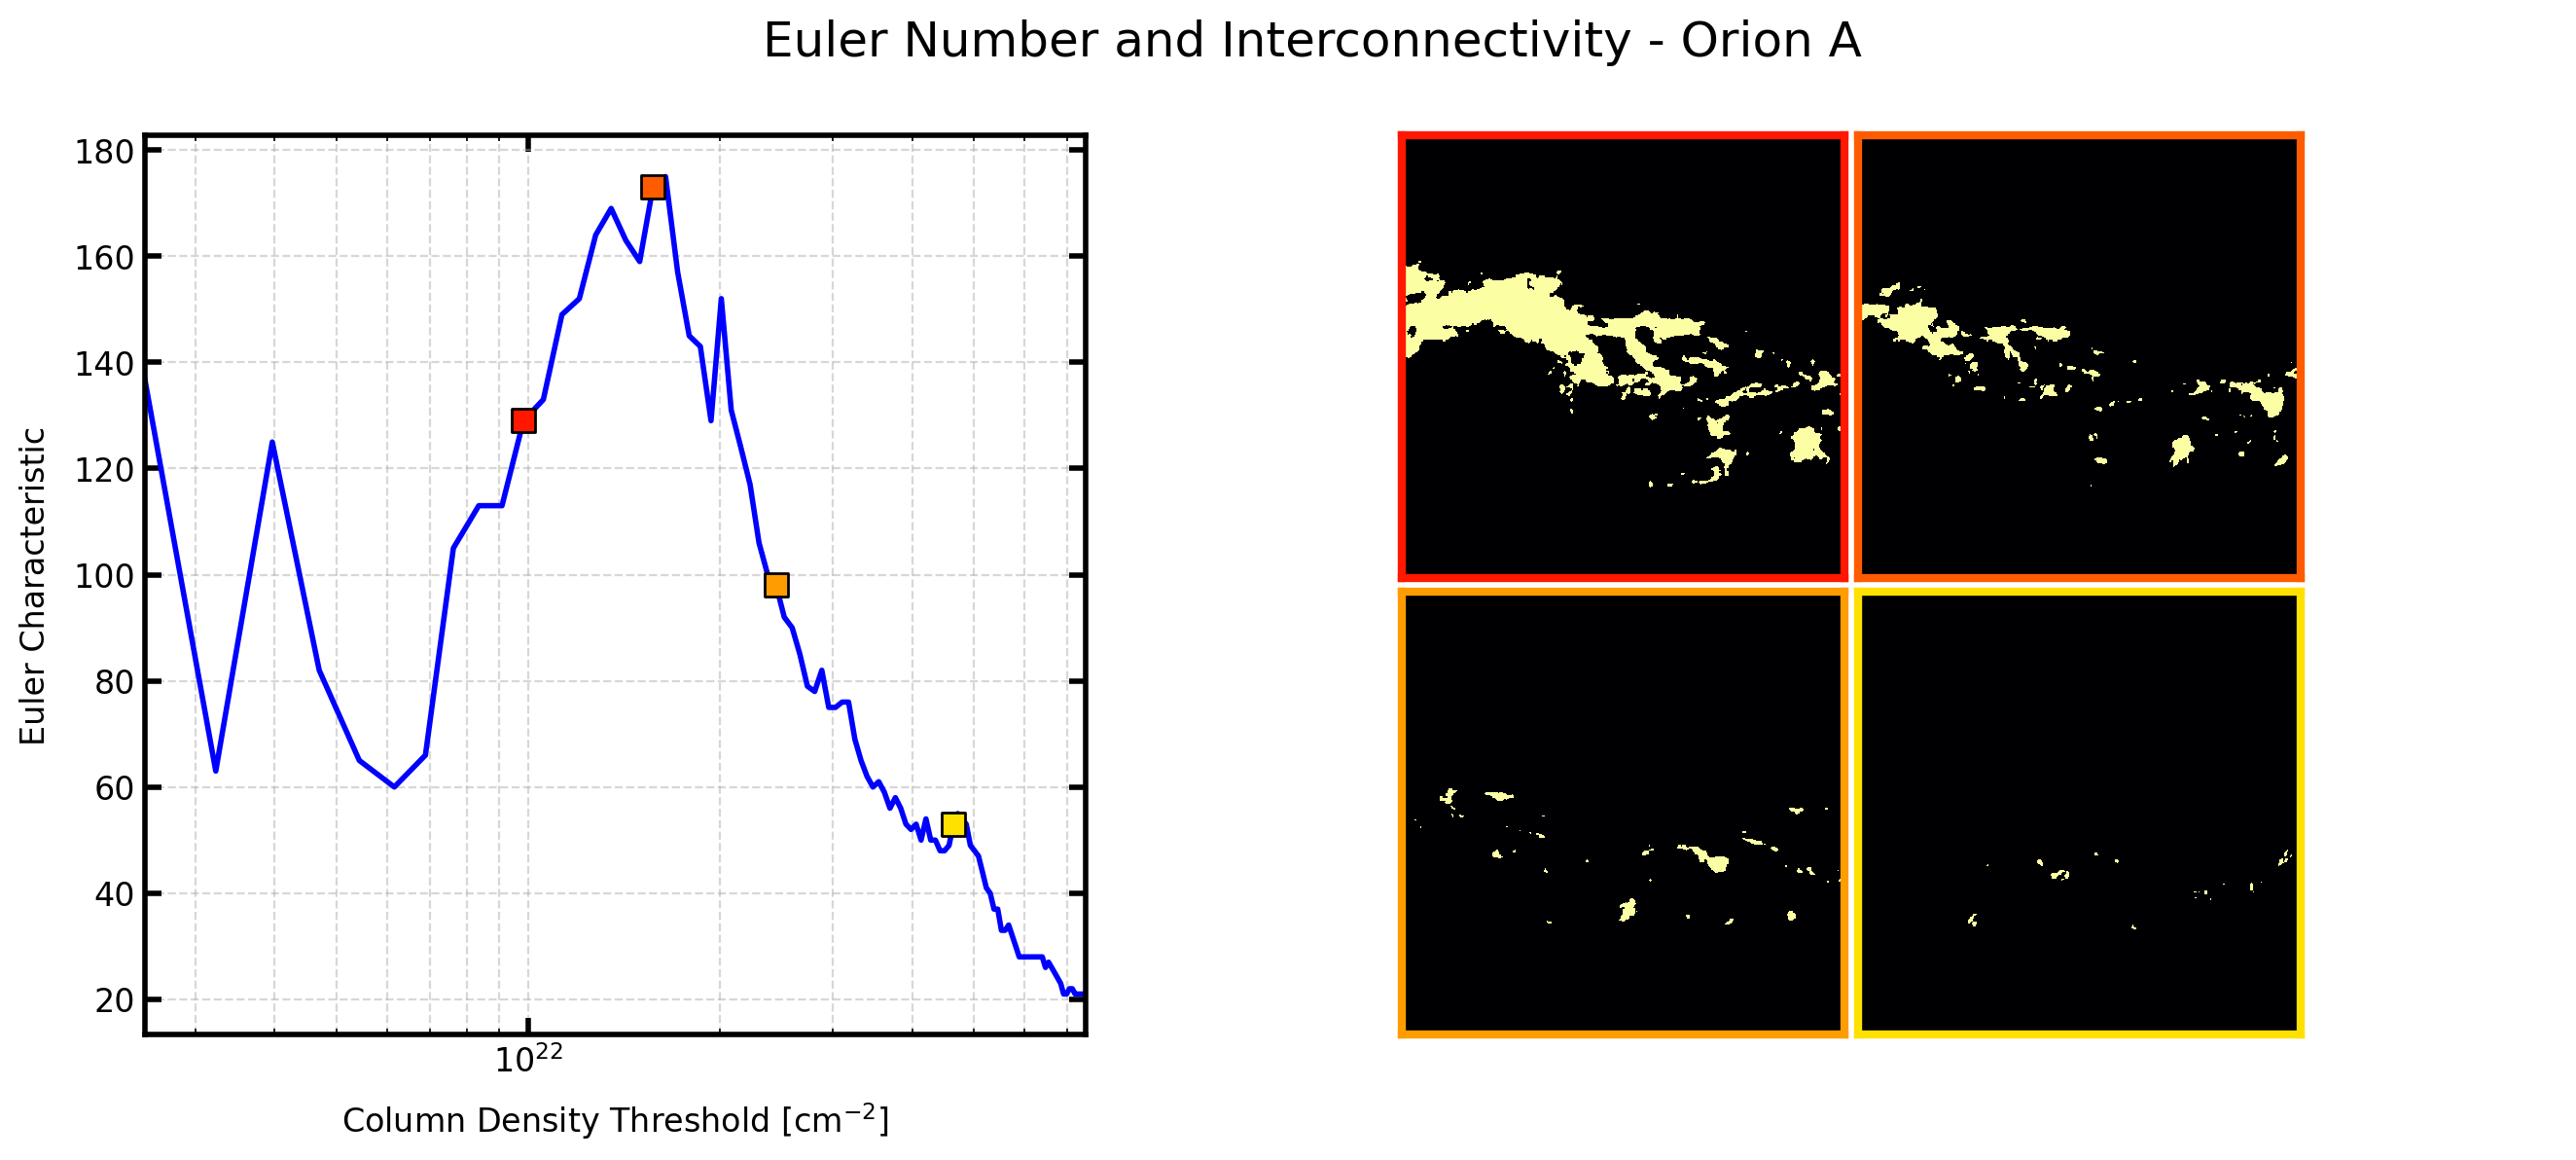
\includegraphics[width=0.65\textwidth]{figures/euler_Orion_A.png}
    \caption{Euler characteristic as a function of column density (left) and four examples of structures (right) marked by colored boxes on the graph (Orion A).}
    \label{fig:Euler_Orion_A}
\end{figure}

\begin{figure}[t]
    \centering
    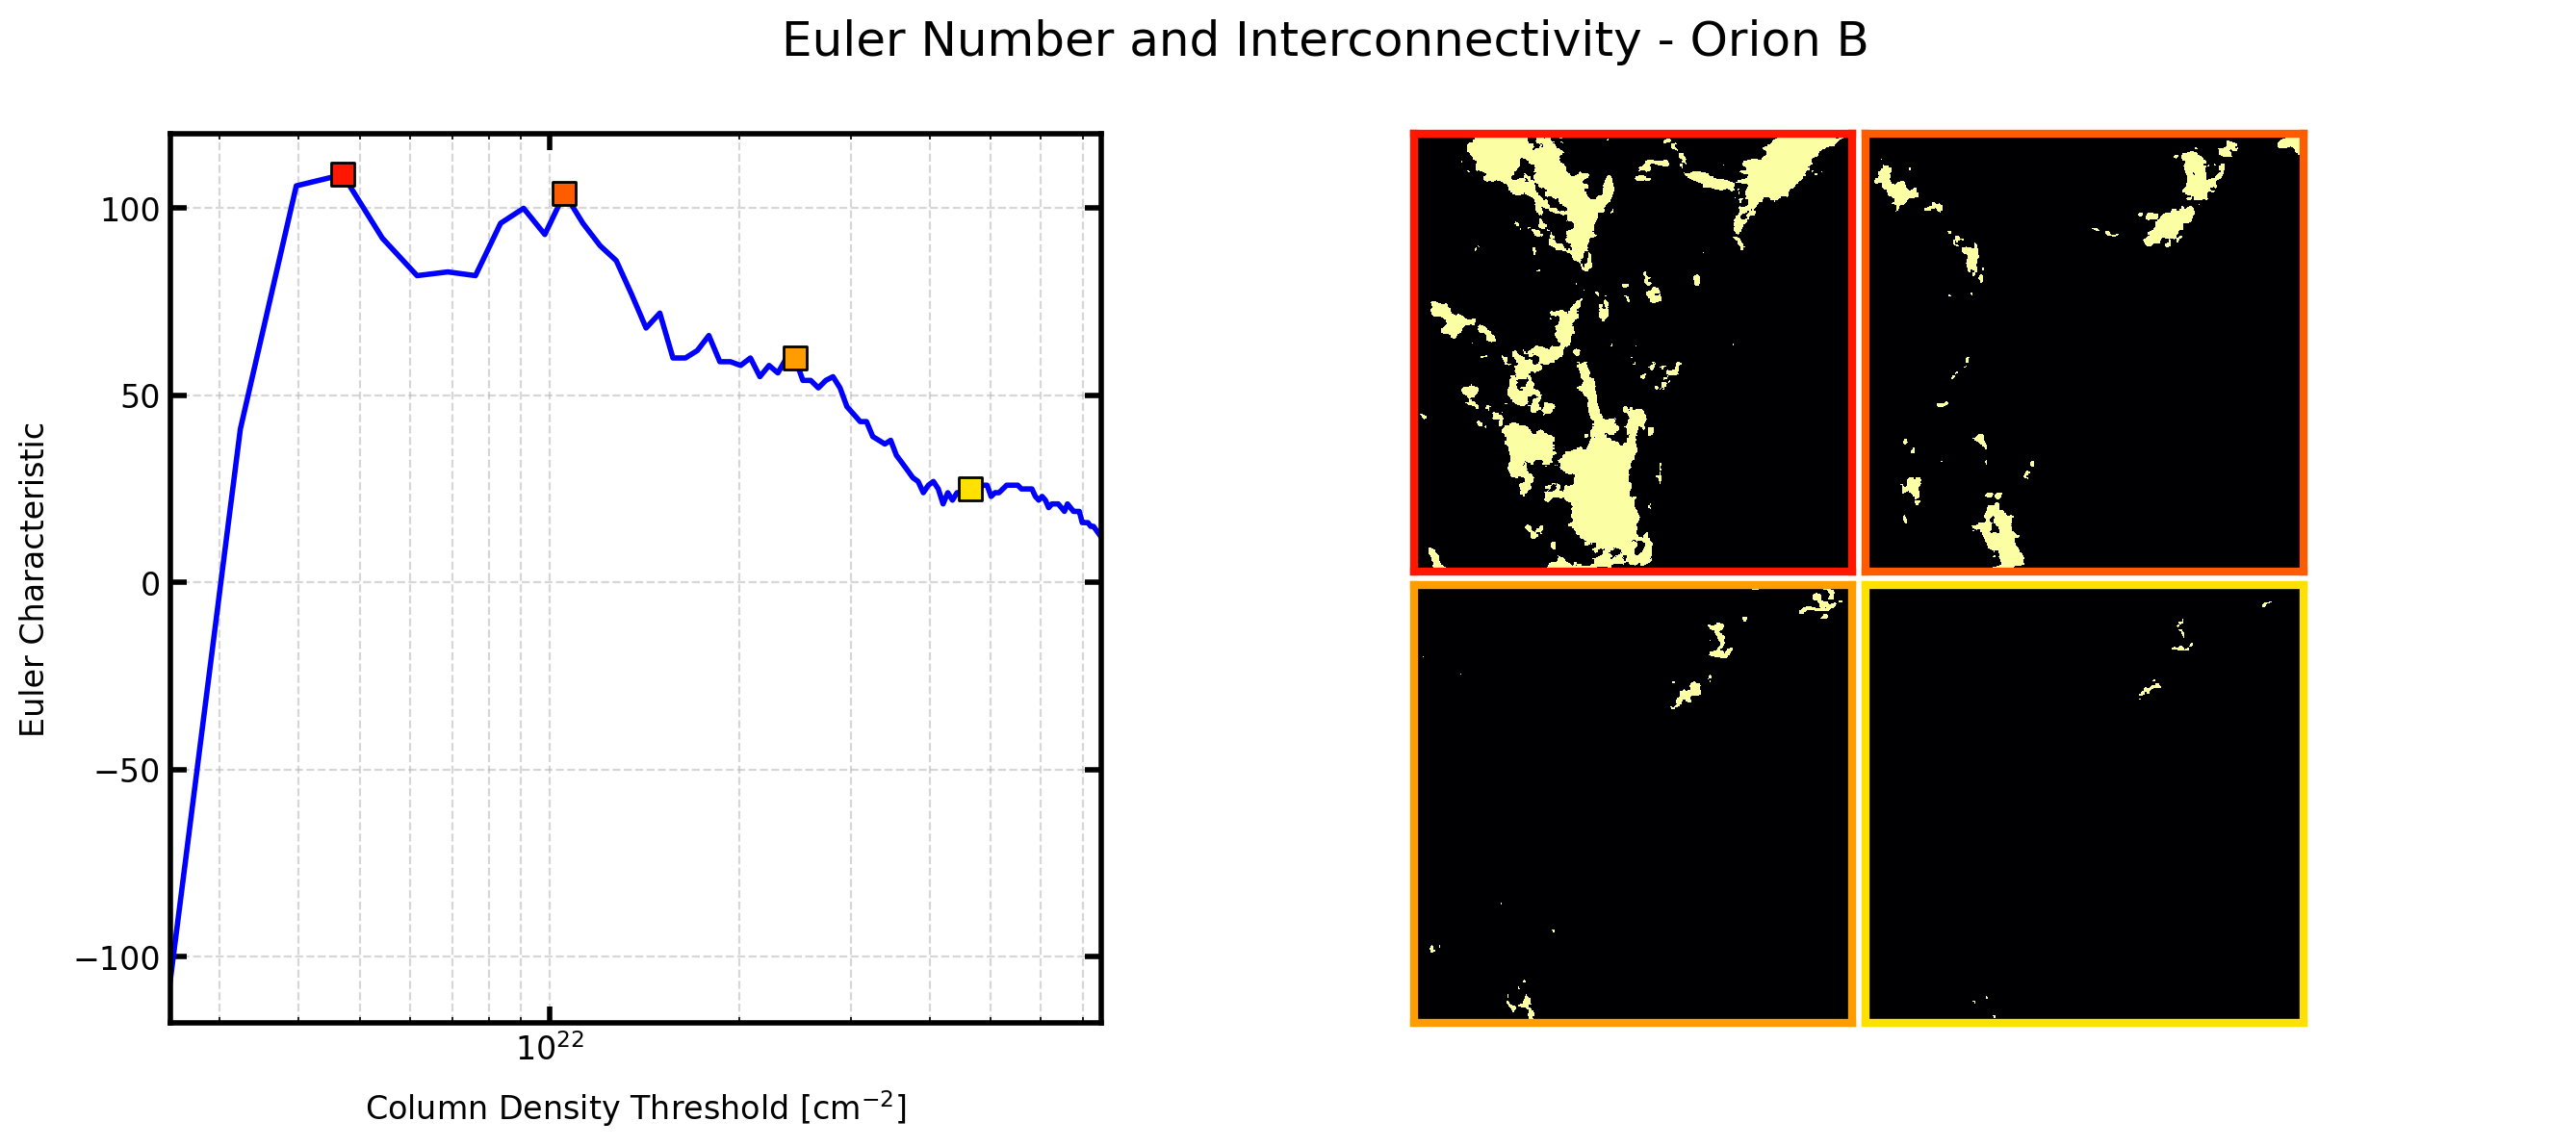
\includegraphics[width=0.65\textwidth]{figures/euler_Orion_B.png}
    \caption{Euler characteristic as a function of column density (left) and four examples of structures (right) marked by colored boxes on the graph (Orion B).}
    \label{fig:Euler_Orion_B}
\end{figure}

% Bring in the MSD plane and individual-structure analysis.

% Connect to star formation.

% End with a synthesis.


% Global Fractal Dimension 
% Orion B is more turbulent and we can defo see that 
% Orion A double fit -> the changing point is where stars from
% We see that point also in the Euler Characteristic
% Less so in Orion B, this gives a coherent picture of how the Minkowski functionals can describe the physics of the cloud.
% Reference that one paper for the local fractal dimension

comparison with the M**alpha method

Star Formation: method a bit limited by the number and extent of the objects.